\section{Bloomberg Technologies}
\subsection{Finalcial Anylytics - Fix Income Pricing and Risk}
git clone --recursive when clone repos with submodules.\\
Maven is like Jave version Plink. Mave projects need pom.xml
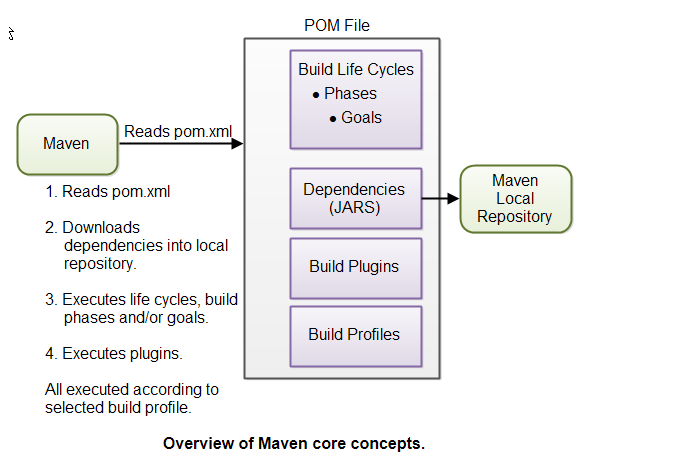
\includegraphics[width=0.5\textwidth]{pics/maven}
nm -- list symbols from object file \\
nm a.out | grep main\\
jenkins groovy function name is the same with file name.\\
In the following makefile, it also has a macro defined for any libraries you want to include, such as the math library -lm. This makefile should be located in the src directory. Note that it also includes a rule for cleaning up your source and object directories if you type make clean. The .PHONY rule keeps make from doing something with a file named clean.
\begin{lstlisting}
IDIR =../include
CC=gcc
CFLAGS=-I$(IDIR)

ODIR=obj
LDIR =../lib

LIBS=-lm

_DEPS = hellomake.h
DEPS = $(patsubst %,$(IDIR)/%,$(_DEPS))

_OBJ = hellomake.o hellofunc.o
OBJ = $(patsubst %,$(ODIR)/%,$(_OBJ))


$(ODIR)/%.o: %.c $(DEPS)
	$(CC) -c -o $@ $< $(CFLAGS)

hellomake: $(OBJ)
	gcc -o $@ $^ $(CFLAGS) $(LIBS)

.PHONY: clean

clean:
	rm -f $(ODIR)/*.o *~ core $(INCDIR)/*~
\end{lstlisting}

make -C change to a directory before doing anything else;\\
xargs build and execute the command line.\\
under many other Unix-like systems, arbitrarily long lists of parameters cannot be passed to a command, so the command may fail with an error message of \"Argument list too long\" (meaning that the exec system call\'s limit on the length of a command line was exceeded): rm \$(find /path -type f)\\
find /path -type f -print | xargs rm
\bigskip\newline
$\bullet$   {\color{red}IntelliJ} will offer the option to create new class in the new menu, only if you right click within the part of your project structure, which is marked as Sources root or Test sources root.  right click the src/main directory in the project structure view and select Mark directory As/Sources Root. That should fix it.\bigskip
\newline
$\bullet$ {\color{green}Zookeeper Introduction} \url{https://www.ibm.com/developerworks/cn/data/library/bd-zookeeper/index.html}
\newline$\bullet$ context in Mapper Class is the medium to contact with hdfs or other compents in Hadoop.
\newline$\bullet$ mapper output type should be indentical with reducer input type.

\# \textbf{Java}
Set is a parent interface of all set classes like TreeSet, LinkedHashSet etc. HashSet is a class implementing Set interface. Set interface is the same.

\# \textbf{Maven}
\begin{itemize}
\item Build elements handle plugins
\item maven-jar-plugin need to specify manifest in which main class is claimed.
\item maven-compiler-plugin is needed to configured to use java vaersion 7 or higher to get rid of Maven Compilation Error: (use -source 7 or higher to enable diamond operator)


\end{itemize}
